\capitulo{5}{Aspectos relevantes del desarrollo del proyecto}

En esta sección de la memoria se mostrará las diferentes fases de maduración y evolución por las que ha pasado el proyecto, haciendo especial hincapié en las dificultades encontradas a la hora de afrontar distintas tareas. También se mostrarán los resultados obtenidos en el estudio.

\section{Evolución temporal}

\subsection{Inicio y motivación}

A principios de curso, tuve la oportunidad de realizar las prácticas curriculares en la consultoría informática local CSA, más concretamente en el departamente de Business Intelligence. Ahí estuve trabajando durante meses con distintas herramientas de la categoría ETL que me resultaron prácticas e interesantes. Por lo que una vez finalizadas las prácticas, le propuse a mi tutor de las mismas la posibilidad de realizar mi trabajo de fin de grado sobre algo relacionado con el tratamiento de datos. Y así llegamos a la conclusión de empezar a trabajar con las herramientas ElasticSearch, Kibana y Logstash, que cumplían el papel de las tres fases de un proceso ETL.

La intención en este proyecto siempre fue desde el principio un estudio de estas herramientas ELK en el que se representerán situaciones que pudieran ocurrir en un entorno real. Por lo que desde un inicio, se pensó en plantear distintos escenarios en función de la manera en la que se ingestaban los datos.

El primer interrogante que se planteó por parte del tutor, Jesus Manuel Maudes Raedo, fue el de investigar que posibilidades ofrecía Logstash a la hora de ingestar, filtrar y exportar datos. En un principio, la idea se antojaba sencilla pero debido a que estos programas son novedosos y no han tenido tanto impacto (aún) como otros como puede ser PowerBI, la documentación presente en Internet sobre conceptos relacionados con este programa era escasa y en su mayoría en lengua anglosajona. Por lo que se comenzó desde lo más básico, tutoriales y guías tanto de plataformas como YouTube, como de las páginas oficiales de Elastic. 

La familiarización con el programa Logstash llevó un gran lapso de tiempo, por lo que se compaginó con investigar el funcionamiento de los plugins que ofrece Elastic desde su \textit{marketplace}, comprender como se podía realizar integraciones con \textit{Python} en el ecosistema Elastic, y estudiar la posibilidad de integrar \textit{machine learning} en el análisis de los datos, y este fue el siguiente punto que se tocó en profundidad.

En este periodo, se completó el primero de los escenarios a analizar y más sencillo, el de importar directamente un fichero de tipo CSV a Elastic. El fichero elegido fue uno que incluía datos sobre los pasajeros del Titanic y que ofrecia la posibilidad de mostrar diferentes herramientas que nos ofrece Kibana a la hora de mostrar los datos.
También se analizó un ejemplo de datos que nos ofrece Elastic que permite explotar al máximo las capacidades de analisis de Kibana. Se trata de los datos de una empresa electrónica que se dedica al comercio de artículos, y gracias a este escenario se pudo comprender con mayor facilidad el funcionamiento de Kibana de cara a desarrollar los siguientes escenarios que se avecinaban.

\paragraph{}
\paragraph{}
\paragraph{}
\paragraph{}
\paragraph{}


\subsection{Cronología de los experimentos}

\subsubsection{Machine Learning}

Habiendo pasado ya un mes desde el comienzo del estudio, la posibilidad de integrar análisis de datos con \textit{machine learning} se antojaba fundamental, pues a priori era una función de pago que ofrece Elastic, por lo que esa vía de integración quedó descartada.

Se introdujo la idea de trabajar con la biblioteca de aprendizaje automático de código abierto \textit{Scikit-Learn}. Para el segundo sprint del proyecto, se giró entorno al estudio, comprensión e investigación de esta biblioteca que se consiguió integrar a través la herramienta \textit{Jupyter Notebook}, en la que se realizaron distintos scripts de pruebas para comprender el funcionamiento de los algoritmos de clasificación, regresión, clustering y reducción de características sobre el \textit{dataset} Iris, un popular conjunto de datos empleado como ejemplo de la utilidad del \textit{machine learning} en el análisis de los mismos. Este conjunto de datos ya lo tenemos almacenado en Elastic, y es desde donde lo cargamos al script para poder trabajar sobre esa información. Una vez los los algoritmos los han procesado, estos datos son ingestados en índices indivuales en ElasticSearch. Una vez se hubo finalizado la carga de los resultados, estos fueron expuestos en un \textit{dashboard} en la herramienta visual Kibana. 

Al no haber cursado la asignatura optativa de Minería de Datos, este proceso de aprendizaje fue costoso y ocupó un gran período de tiempo hasta que se comprendieron de manera correcta los conceptos tratados.

También se mencionó la posibilidad de realizar funciones como Map Reduce en algún momento del ETL, y se dedicó un tiempo a investigar en qué momento y en qué herramienta era más óptimo implementar esta función. 

\paragraph{}
\paragraph{}
\paragraph{}
\paragraph{}
\paragraph{}

\subsubsection{Data Streams}

Con lo mencionado anteriormente se finalizó el segundo sprint y dieron comienzo los dos siguientes, en los que la misión principal fue la de estudiar el funcionamiento de los \textit{streams} de datos, cómo funcionan y de qué forma los podemos ingestar en Elastic.

El tutor de este proyecto proporcionó distintas fuentes para encontrar \textit{streamings} de datos con los que poder experimentar y estudiar las posibilidades reales que ofrecen. Se continuó por un repositorio de GitHub de nombre \href{https://github.com/ColinEberhardt/awesome-public-streaming-datasets}{awesome public streaming datasets} en el que se incluían distintas interfaces via \textit{WebSockets} de \textit{data streams}. El problema venia dado cuando queríamos ingestar estos \textit{streamings} con Elastic, ya que bastantes de las APIs que se ofrecían eran complejas, y las que no, ofrecían envios de datos muy básicos. A todo esto se le suma que no habiendo cursado la asignatura de Sistemas Distribuidos, en la cuál se estudia el funcionamiento de los \textit{WebSockets} detenidamente, me supuso un mayor tiempo para la compresión de estos conceptos.

Por lo que se optó por una opción que era gratuita y satisfacia en gran parte los requisitos que se pedían: la \textit{RESTful API} y \textit{WebSocket} de la empresa de operaciones de criptomonedas \textbf{Finnhub}.

Gracias a la guía que presentan su \href{https://finnhub.io/docs/api/websocket-trades}{página web}, y los diferentes tutoriales y documentación presente en Internet, se consiguió desarrollar un script en Python que se suscribiese al \textit{stream} de datos y mandará los datos directamente a Elastic, sin realizar ninguna operación intermedia, completando así otro de los escenarios tratados.

En vista de que existía la posibilidad de realizar alguna manipulación o transformación a los datos originales que Finnhub mandaba, se optó por generar un script que modificará el nombre de las variables y mandará a Logstash los datos del \textit{stream} para poder realizar más filtros desde allí. El envío de datos del script a Logstash se realiza a través del protocolo de red HTTP, a través del puerto 8080 más concretamente.

Una vez los datos llegan a Logstash, se les realiza unas modificaciones, omitiendo el envío de campos vacíos, modificando el tipo de las variables para que sean legibles por Elastic, y generando nuevos campos en base a los originales relizando operaciones sobre ellos. Una vez que los filtros se realizan los datos procesados por Logstash son mostrados por pantalla y enviados a Elastic para que desde allí puedan ser ilustrados y expuestos a través de Kibana, dando fin así a otro de los posibles escenarios analizados.

Cabe remarcar que al encontrar dificultades en el envío de datos a través de las fuentes del repositorio mencionado, se estudió paralelamente la posibilidad de mandar los datos con la herramienta \textit{Filebeat}, la cuál ofrece una integración sencilla con Elastic pero teniendo acceso a \textit{streamings} de datos más complejos. Por lo que añadir esta opción hubiera sido aumentar la carga de trabajo, por lo que se deja como posible mejora de cara a trabajos futuros.

\section{Resultados del estudio}

\subsection{Introducción}
Una vez maduradas las posibilidades que ofrece el sistema ELK, se ha decidido estructurar este apartado en varios, en función de las conclusiones sacadas. Se hará hincapié en los conceptos teóricos mencionados previamentes como pueden ser MapReduce o Machine Learning entre otros.

\subsection{ELK con Elastic en la nube}

Elastic ofrece la versión de trabajo \textit{cloud}, en la que se dispone de un espacio de almacenamiento para los distintos índices de datos de manera que se puedan trabajar con ellos desde distintas ubicaciones. Esta funcionalidad es ofrecida pagando un precio efectivo, por lo que no lo contemplamos como posibilidad de trabajo. Pero de forma gratuita, Elastic pone a servicio del usuario diversas fuentes de datos en su nube para poder experimentar y aprender a sacar el máximo potencial tanto a ElasticSearch como a Kibana.

Tras evaluar la situación, se llegó a la conclusión de que los datos utilizados en los diferentes escenarios permitían a Kibana mostrar parte de su potencial, pero no todo. Por lo que para mostrar la herramienta al completo se utilizaron datos que nos ofrece Elastic a modo de ejemplo.

En este caso, se eligieron los datos sobre un \textit{e-commerce} el cuál recibe pedidos de todo el mundo y de distintos tipos. Permitiendo así poder mostrar visualizaciones de mapas, histogramas y demás funciones avanzadas, como pueden ser los distintos gráficos de líneas para evaluar la evolución de los gastos por categorías o gráficos de barras en lo que se muestra la evolución de las ganancias a lo largo de un marco temporal.

\begin{figure}
    \centering
    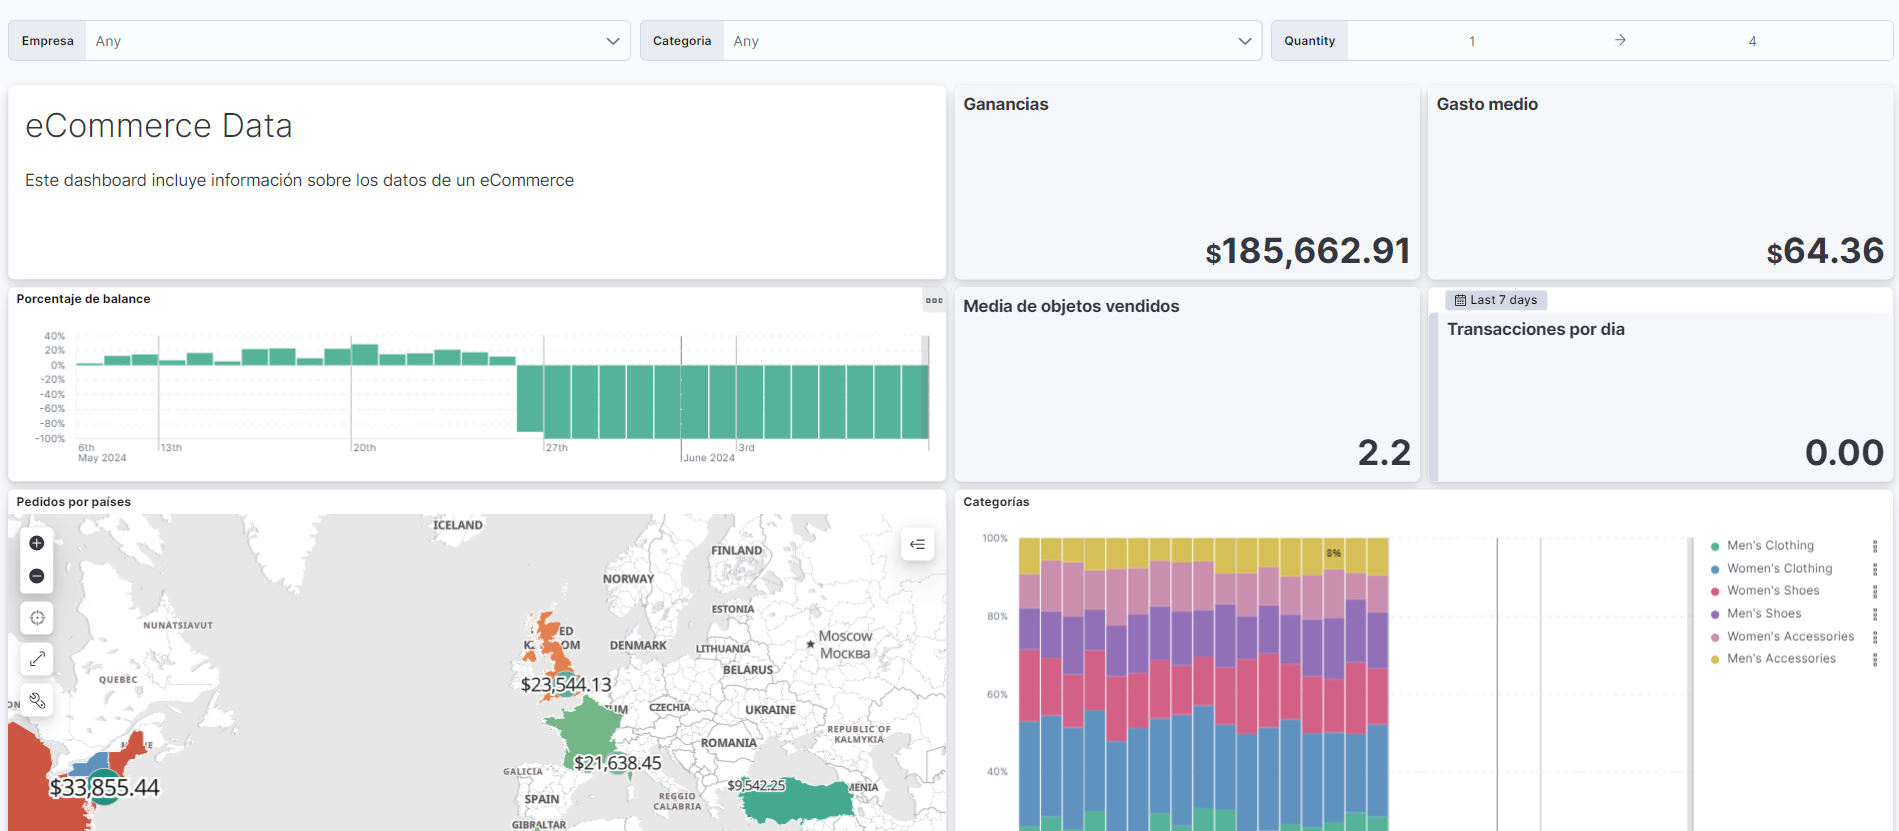
\includegraphics[width=1\linewidth]{img/escenario6.png}
    \caption{Dashboard final}
    \label{fig:escenarioNube}
\end{figure}

\paragraph{ }
\paragraph{ }
\paragraph{ }
\paragraph{}
\paragraph{}
\paragraph{}
\paragraph{}
\paragraph{  }
\paragraph{  }
\paragraph{  }
\paragraph{  }
\paragraph{  }


\subsection{Escenarios de ingesta de datos}

En este apartado se hará un desglose de los diferentes escenarios de ingesta de datos de diversas fuentes sobre los que se ha trabajado en este estudio incluyendo su desarrollo y resultados finales obtenidos.

\subsubsection{Escenario 1: ingesta desde fichero en Elastic}
Este primer escenario es el más simple de todos, consiste en la importación de un fichero local a Elastic a través del servicio de importación de datos básico que se ofrece.

El archivo que se va a analizar recibe el nombre de \textit{titanic.csv}, es un archivo de valores separados por comas que muestra datos sobre los pasajeros que formaban parte de la tripulación del hundido barco \textit{Titanic}.
Es un archivo interesante como punto de partida para entender el funcionamiento de las herramientas software empleadas.

Teniendo este archivo en el sistema local, en el apartado que dice "import from file", y desde ahi se selecciona el mencionado CSV. Una vez que lo seleccionado, Elastic cargará los datos y se podrán visualizar desde la pestaña \textit{Discover}, en la que aparecerán las filas del fichero. Desde aquí se pueden clasificar y filtrar de manera que se pueda comprobar que los datos han sido cargados correctamente.

Una vez tenemos los datos cargados, ya se puede crear el \textit{Dashboard} pertinente accediendo a la pestaña \textit{Visualize} y desde aquí a \textit{Dashboard}. Una vez ahí, se seleccionará cuál es la fuente que proveerá de datos las visualizaciones, seleccionamos la del archivo que se acaba de importar, y ya se podrá empezar a generar visualizaciones.

La estructura básica estará formada por un texto descriptivo del \textit{dashboard} en formato Markdown incluyendo datos del autor, así como descripciones de las distintas visualizaciones presentes. Este elemento es fundamental en todo \textit{dashboard} cumpliento el papel de introducción a la hora de la toma de contacto con el contexto de las visualizaciones.

En el \textit{dashboard} resultante se han añadido gráficos de las edades  (ver ilustración  \ref{fig:barras1}), los géneros, métricas  (ver ilustración  \ref{fig:metricas1}), y gráficos de donut  (ver ilustración  \ref{fig:donut1}) en función de la clase del pasajero, la cuál se puede filtrar en función de lo que interese desde la barra superior dónde están presentes los diferentes filtrados que se pueden hacer por género del pasajero, edad de los mismos, por que puerta de embarque accedieron, la clase de su billete o si sobrevivieron  (ver ilustración  \ref{fig:escenario1}).

\begin{figure}
    \centering
    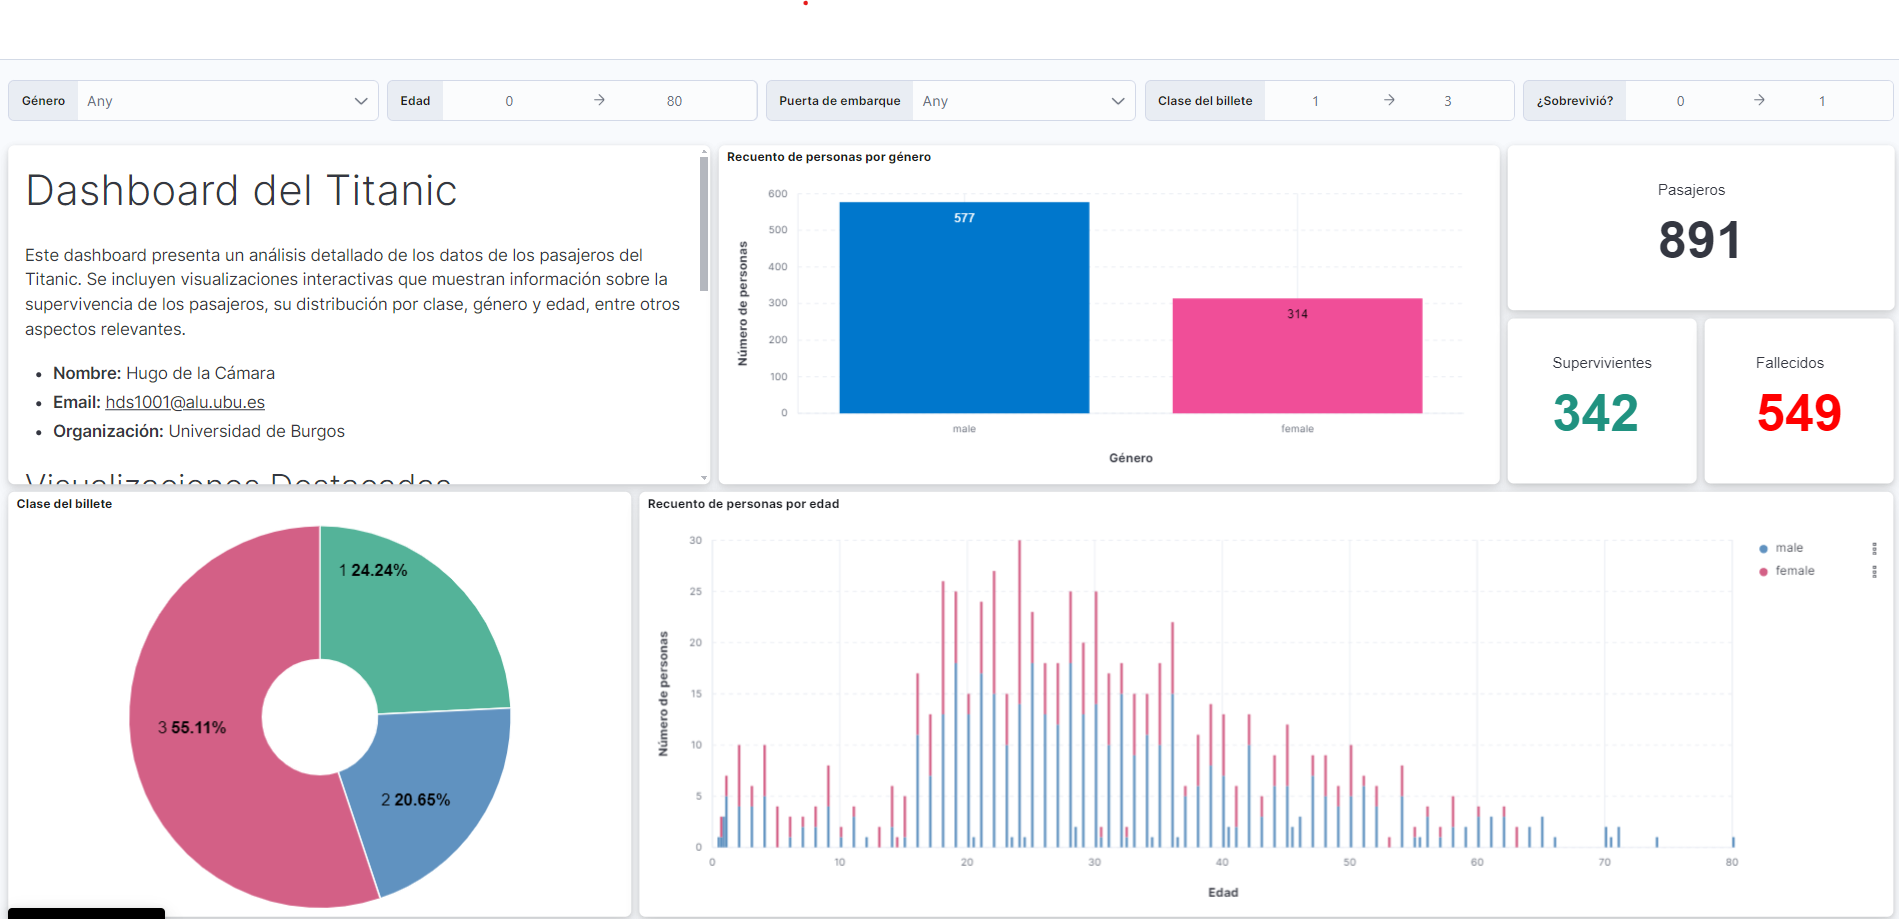
\includegraphics[width=1\linewidth]{img/escenario1.png}
    \caption{Dashboard final del primer escenario}
    \label{fig:escenario1}
\end{figure}

\begin{figure}
    \centering
    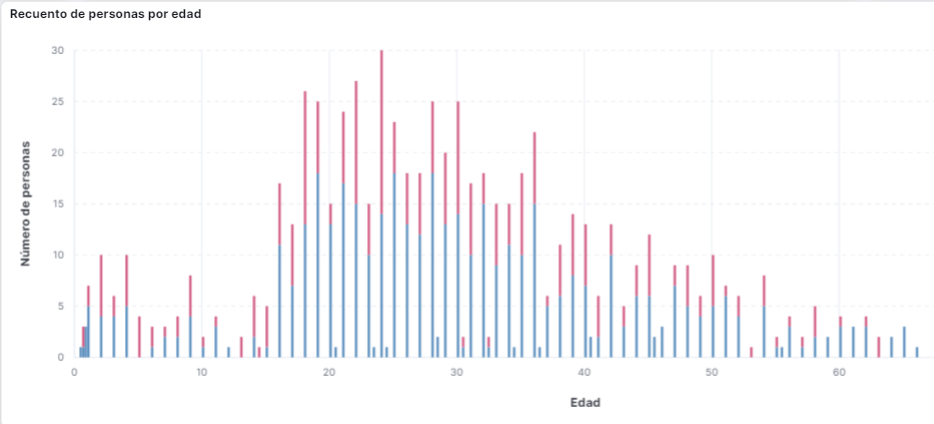
\includegraphics[width=1\linewidth]{img/edades.png}
    \caption{Gráfico de barras por edades y género}
    \label{fig:barras1}
\end{figure}


\begin{figure}
    \centering
    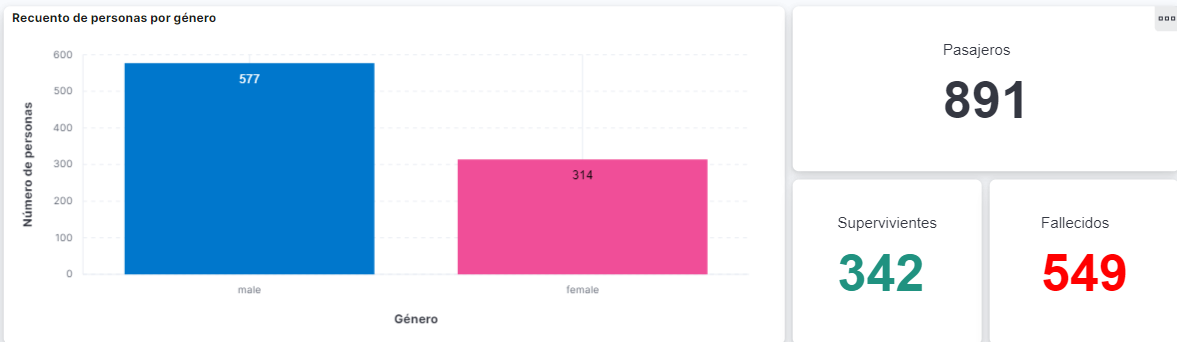
\includegraphics[width=1\linewidth]{img/graficos1.png}
    \caption{Métricas en función del filtrado}
    \label{fig:metricas1}
\end{figure}

\begin{figure}
    \centering
    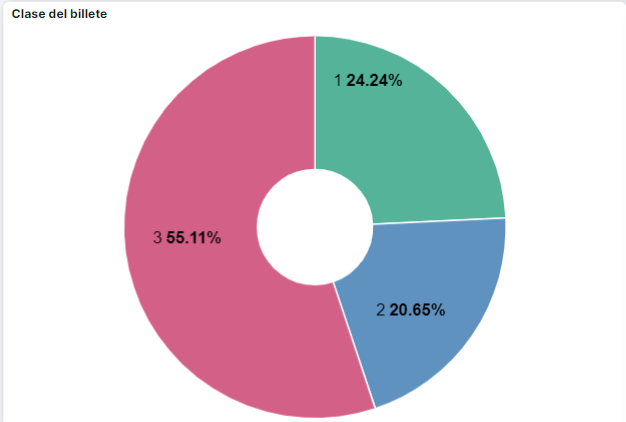
\includegraphics[width=1\linewidth]{img/donut.png}
    \caption{Gráfico de donut en función de la clase del billete}
    \label{fig:donut1}
\end{figure}

\paragraph{}
\paragraph{}
\paragraph{}
\paragraph{}
\paragraph{}
\paragraph{}
\paragraph{}
\paragraph{}

\subsubsection{Escenario 2: ingesta desde fichero con Logstash}

Este segundo caso, es una modificación del primero, lo que se pretende es importar un archivo presente en el sistema en Logstash, realizarle una serie de modificaciones y cargar esos datos tratados en Elastic para poder visualizarlos en Kibana.

El archivo sobre el que se va a trabajar es uno de tipo \textit{log} que indica las diferentes viviendas ofertadas en una inmobiliaria, incluyendo campos como el número de la casa, la ciudad en la que se ubican, el barrio en el que se encuentra, el precio de la misma, el número de habitaciones que tiene, el número de baños disponibles y los metros cuadrados de la vivienda.

Para trabajar con logstash, se necesita un archivo de configuración para que éste entienda lo se le pide que haga. Este archivo es de tipo \textit{.conf} e incluye 3 apartados:
\begin{itemize}
    \item \textbf{Input}: ruta hacia el archivo que se quiere leer
    \item \textbf{Filter}: operaciones a realizarle a estos datos
    \item \textbf{Output}: salida por pantalla de los datos mandados a Elastic una vez son tratados.
\end{itemize}

En este escenario se le va a dar toda la relevancia al apartado \textit{filter} del fichero de configuración  (ver ilustración   \ref{fig:filter}), que va a ser en el que se realizan las transformaciones de los datos. 

\begin{figure}
    \centering
    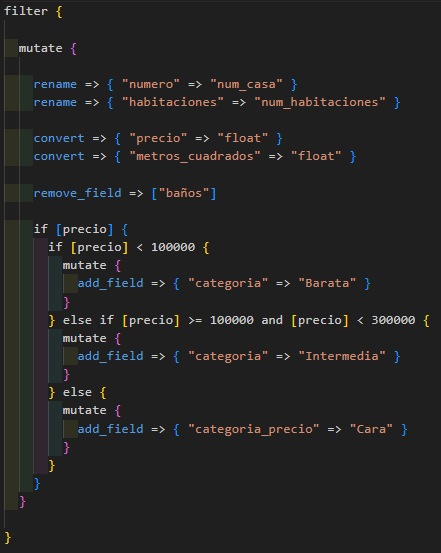
\includegraphics[width=1\linewidth]{img/filter.png}
    \caption{Sección filter del archivo de configuración.}
    \label{fig:filter}
\end{figure}

La primera operación que se va a realizar es la de modificar el nombre de los campos \textit{numero} por \textit{num casa} y de \textit{habitaciones} por \textit{num habitaciones} con la función \textit{rename}  (ver ilustración  \ref{fig:rename}), la cuál permite cumplir esta orden. Esto es de gran utilidad cuándo el nombre de algún campo no deja claro la información que éste ofrece.

\begin{figure}
    \centering
    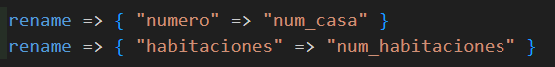
\includegraphics[width=1\linewidth]{img/rename.png}
    \caption{Función que renombra los campos indicados}
    \label{fig:rename}
\end{figure}

La siguiente transformación que se ha aplicado es la de cambiar los tipos de los campos \textit{precio} y \textit{metros cuadrados} con la función \textit{convert}  (ver ilustración  \ref{fig:convert}), la cuál es de gran ayuda cuando los campos que se van a mandar a Elastic no poseen un tipado que permita el correcto procesamiento de la información.

\begin{figure}
    \centering
    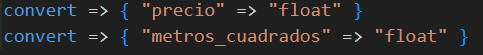
\includegraphics[width=1\linewidth]{img/convert.png}
    \caption{Función que convierte los tipos de los campos indicados}
    \label{fig:convert}
\end{figure}

La tercera operación aplicada en este filtro va a consistir en la eliminación del campo \textit{baños} con la función \textit{remove field}  (ver ilustración  \ref{fig:remove}), la cuál permite eliminar del mensaje final mandado a Elastic contendido que no se considere oportuno o que carece de relevancia.

\begin{figure}
    \centering
    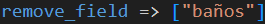
\includegraphics[width=1\linewidth]{img/remove.png}
    \caption{Función en la que se elimina el campo \textit{baño}}
    \label{fig:remove}
\end{figure}
\paragraph{}

La última transformación es una discretización en función del campo \textit{precio} de cada vivienda  (ver ilustración  \ref{fig:discre}). En ella se indica la creación de un nuevo campo para cada registro llamado \textit{categoria}, en el cuál si la vivienda tiene un precio menor de 100000 será considerada de categoría barata, si el precio oscila entre 100000 y 300000 será considerada de categoría intermedia y si excede la última cantidad será catalogada como cara.

\begin{figure}
    \centering
    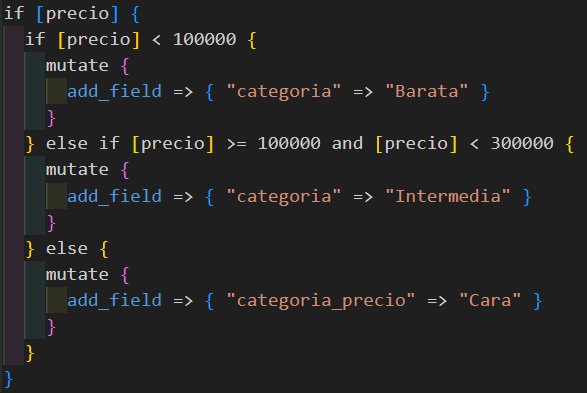
\includegraphics[width=1\linewidth]{img/discretizacion.png}
    \caption{Función en la que se discretiza en función del precio de la vivienda}
    \label{fig:discre}
\end{figure}

Una vez ejecutado Logstash, a Elastic le llega un índice con toda la información que se ha procesado en el filtro. Y una vez se tienen los datos en el entorno, podemos generar el \textit{dashboard}  (ver ilustración  \ref{fig:dashboard2}) para mostrar toda la información.

En este tablero se han incluído visualizaciones como un gráfico de barras en el que se muestra información sobre el número de viviendas por categoría de precio clasificada  (ver ilustración  \ref{fig:barrasViv1}), también una métrica y una tabla que muestran el número total de viviendas  (ver ilustración  \ref{fig:metrica2}), un gráfico de donut mostando el porcentaje de las viviendas que pertenecen a cada ciudad y barrio  (ver ilustración  \ref{fig:donut2}), un gráfico de árbol que muestra la media de metros cuadrados de la vivienda por ciudad  (ver ilustración  \ref{fig:treemap2}) y un gráfico de barras apiladas que muestra el número de viviendas y el número de habitaciones medio por barrio  (ver ilustración  \ref{fig:barrasViv2}).

\begin{figure}
    \centering
    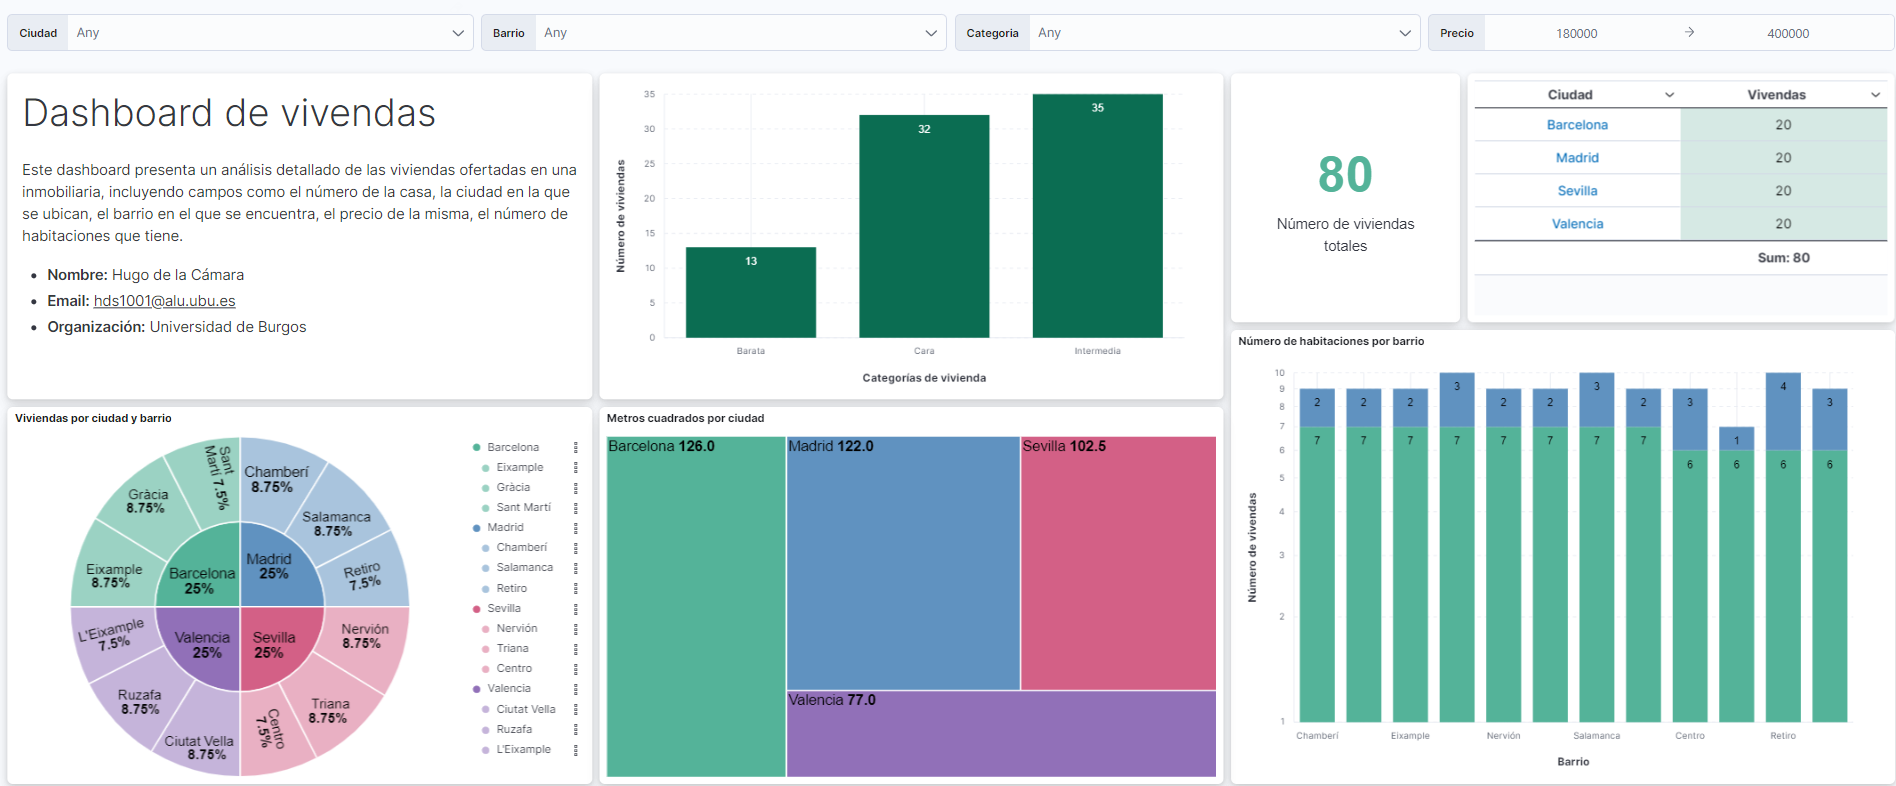
\includegraphics[width=1\linewidth]{dashViviendas.png}
    \caption{Dashboard final del escenario 2}
    \label{fig:dashboard2}
\end{figure}

\begin{figure}
    \centering
    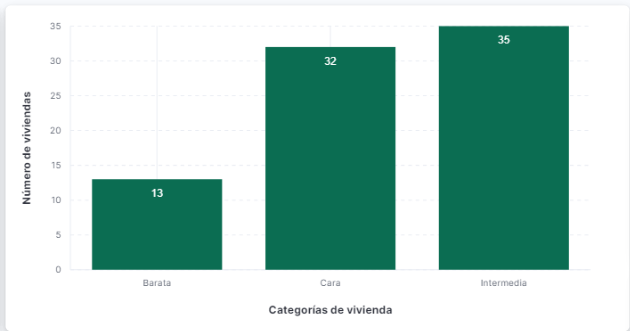
\includegraphics[width=1\linewidth]{img/barrasViv.png}
    \caption{Gráfico de barras del número de viviendas por categoría de precio.}
    \label{fig:barrasViv1}
\end{figure}

\begin{figure}
    \centering
    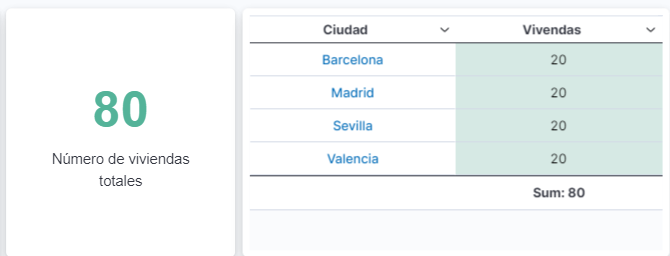
\includegraphics[width=1\linewidth]{img/metricaViv.png}
    \caption{Métrica y tabla del número de viviendas.}
    \label{fig:metrica2}
\end{figure}

\begin{figure}
    \centering
    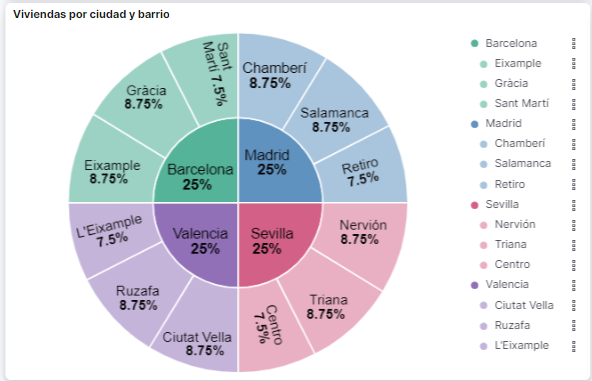
\includegraphics[width=1\linewidth]{img/donutViv.png}
    \caption{Gráfico de donut que muestra el porcentaje de viviendas por ciudad y barrio.}
    \label{fig:donut2}
\end{figure}

\begin{figure}
    \centering
    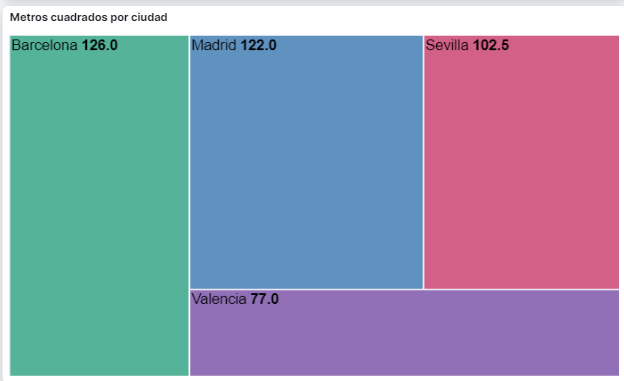
\includegraphics[width=1\linewidth]{img/graficoViv.png}
    \caption{Gráfico de árbol que muestra la media de metros cuadrado por ciudad.}
    \label{fig:treemap2}
\end{figure}

\begin{figure}
    \centering
    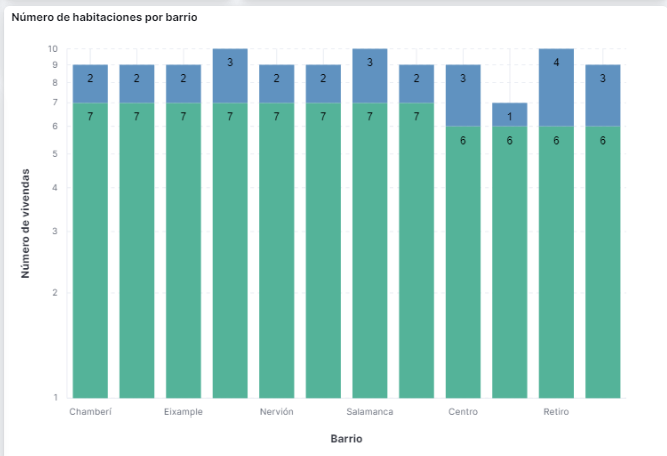
\includegraphics[width=1\linewidth]{img/barras2Viv.png}
    \caption{Gráfico de barras que muestra el número de habitaciones y de viviendas por barrio.}
    \label{fig:barrasViv2}
\end{figure}

\begin{figure}
    \centering
    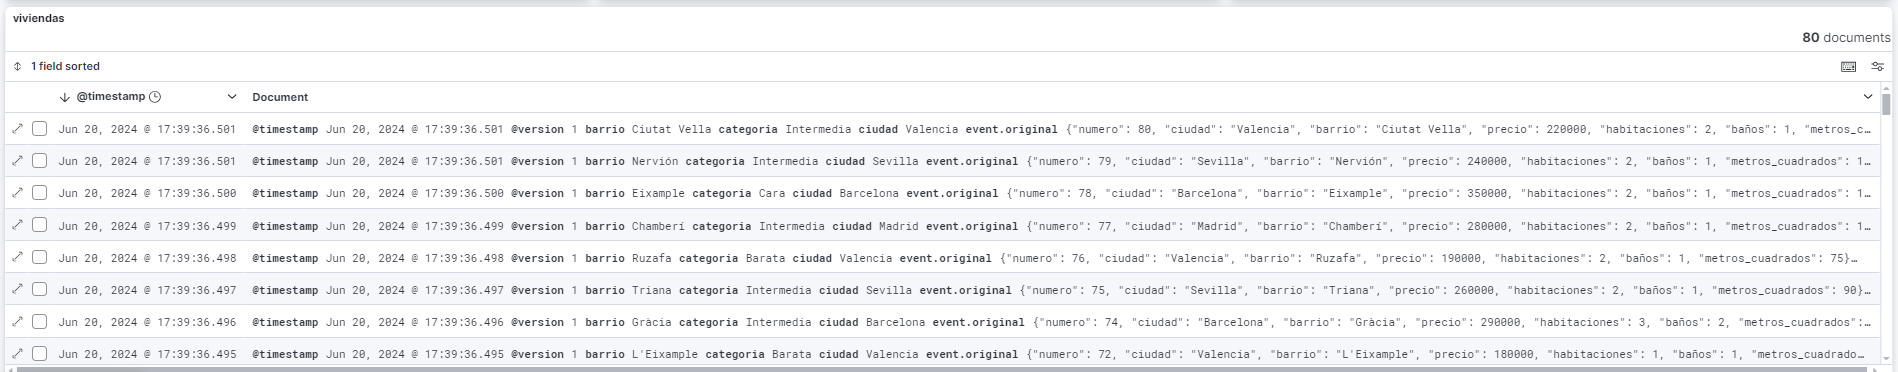
\includegraphics[width=1\linewidth]{img/datosViv.png}
    \caption{Datos del índice del escenario 2}
    \label{fig:datos2}
\end{figure}

\subsubsection{Escenario 3: ingesta a través de WebSocket a Elastic}

El tercer caso se tratará de suscribirse a un data stream a través de la tecnología WebSocket que nos irá mandando datos en tiempo real a Elastic y se irán mostrando en Kibana.

En un principio el tema de los envíos de datos en vivo se planteo como una de las bases del trabajo, puesto que es la situación que más se puede asemejar a un entorno de trabajo con IoT. El problema estaba en que no se disponía de una suscripción a un servicio de ingesta de datos en vivo, por lo que se tuvo que investigar de qué manera se podía implementar esta funcionalidad en el entorno de trabajo. Llegando así al siguiente \href{https://github.com/ColinEberhardt/awesome-public-streaming-datasets}{repositorio} GitHub, el cuál incluía distintos datasets públicos con actualizaciones en vivo.

Tras probar distintos conjuntos de este repositorio, se llegó a la conclusión de que la opción más interesante era la de \href{https://finnhub.io/docs/api/websocket-trades}{Finnhub}, ya que proporciona una \textit{Real-Time RESTful API} y \textit{WebSocket} para interactuar con \textit{stocks} y criptomonedas del mercado.

La \href{https://finnhub.io/}{página oficial} es sencilla de entender, nos proporciona tanto documentación sobre el funcionamiento del \textit{WebSocket}, como una \textit{API key} gratuita para suscribirnos al servicio. Una vez que la tenemos, en la documentación se nos proporciona la estructura básica del script del \textit{WebSocket} escrito en Python. Se debe introducir la \textit{key} obtenida y correr el programa. 

Al ejecutarlo, se mostrara por pantalla las actualizaciones de los distintos precios y características de los símbolos de mercado a los que se haya suscrito en el script. 

En este primer escenario trabajando con \textit{data streams}, la ingesta de datos se hace de la manera más sencilla y estando lo más cerca posible de la fuente de los datos. La información se manda directamente del \textit{WebSocket} a Elastic a través del puerto 9200, llegando al índice "websocket-data", donde los datos en vivo son almacenados, de manera que se pueda usarlos en Kibana para exponerlos y analizarlos en un \textit{dashboard}.

\begin{figure}
    \centering
    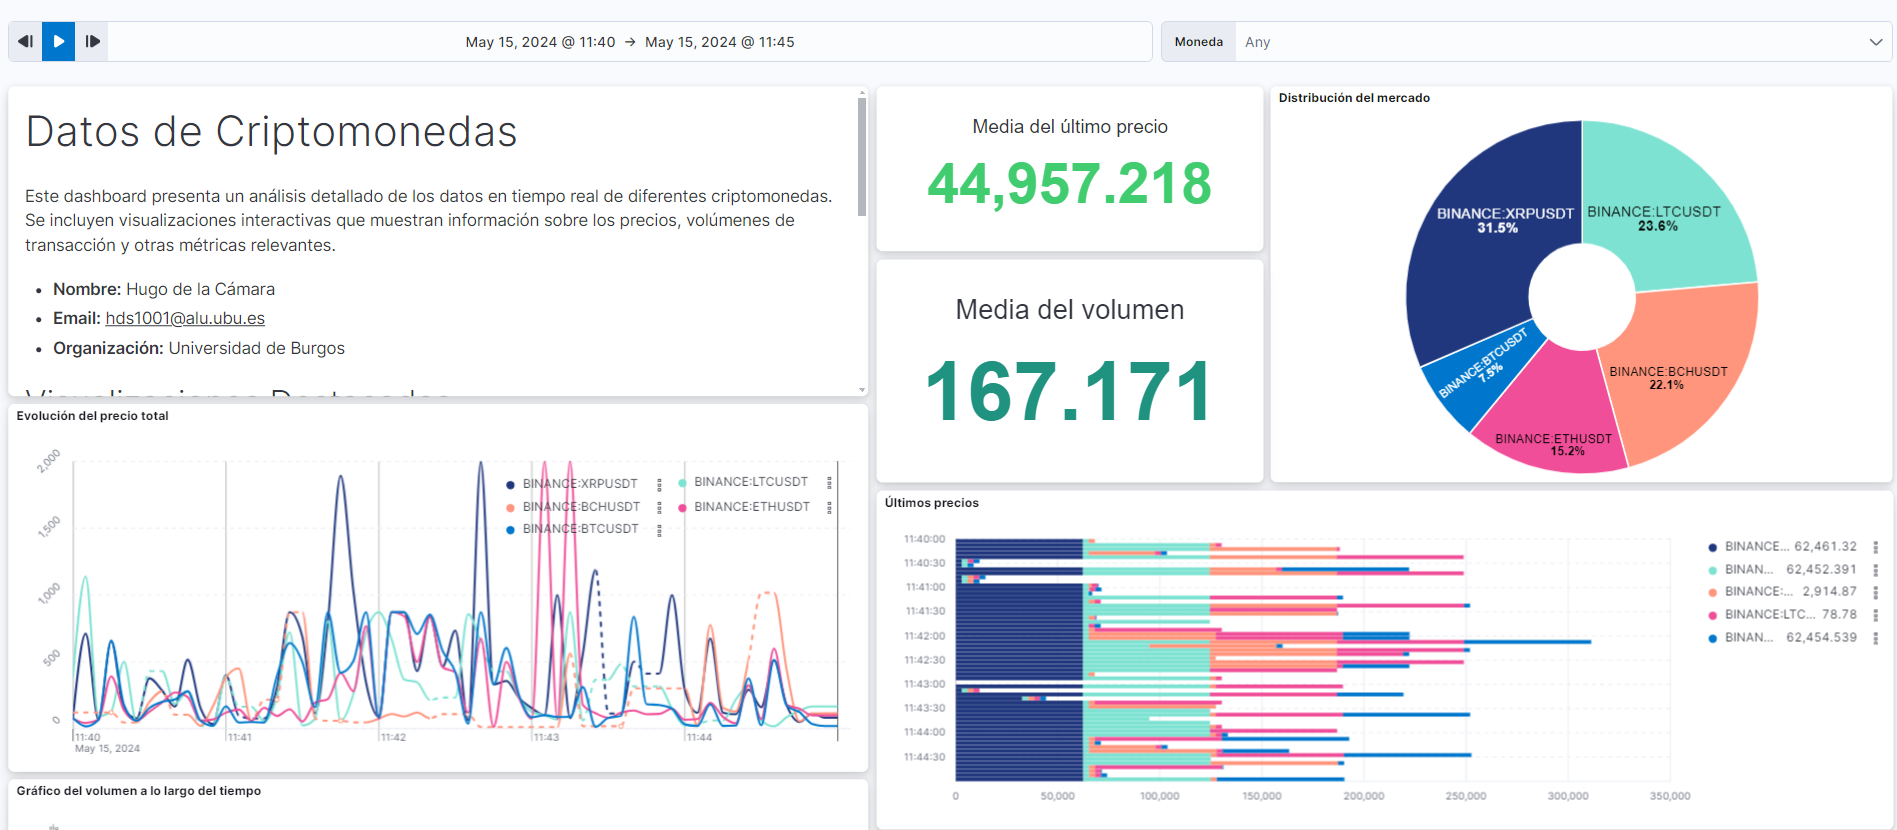
\includegraphics[width=1\linewidth]{img/escenario4-1.png}
    \caption{Dashboard final del tercer escenario}
    \label{fig:escenario3}
\end{figure}
\paragraph{ }
\paragraph{ }
\paragraph{ }
\paragraph{ }
\paragraph{ }
\paragraph{ }
\paragraph{ }
\paragraph{ }
\paragraph{ }
\paragraph{ }
\paragraph{ }
\paragraph{ }
\paragraph{ }
\paragraph{ }
\paragraph{ }

\subsubsection{Escenario 4: ingesta a través de WebSocket con Logstash}

En este cuarto escenario se pretendió rizar el rizo del anterior, y estudiar la posibilidad de modificar esos datos mandados por el WebSocket a través de Logstash antes de mandárselos a Elastic.

Teniendo Logstash presente en el sistema ELK, resulta interesante ver las posbilidades que ofrece a la hora de filtrar y modificar datos en vivo con el apoyo de la documentación presente sobre el tema tanto en la web oficial de Elastic como en foros como StackOverflow.

Para ello, se utilizará el \textit{data stream} del script del tercer escenario, sobre el que se realizarán una serie de modificaciones. La primera va a ser en el mensaje que se manda a Logstash, puesto que las variables sobre cada \textit{stock}, eran mandadas con una letra identificatoria, las cuales sin tener conocimientos sobre el tema, no son comprensibles. Así se modificó la forma en la que se mandaban, cambiando la letra por el nombre completo de la variable en cuestión. 

Tras esto, la siguiente modificación era cambiar el destino de los datos, el cuál ahora iba a ser Logstash. Se utilizó HTTP para realizar este envío en lugar de al puerto 9200 (Elastic) al 8080, en el cuál está Logstash a la escucha de eventos. Con estas modificaciones, al ejecutar el código, los datos son mandados a Logstash para continuar el tratamiento allí.

En Logstash, se aplicaron cambios al mensaje final, eliminando campos vacíos para ahorrar volumen de información, modificando el tipo de las variables para poder realizar posibles operaciones con ellas de manera más sencilla con datos de tipo \textit{float} e \textit{integer}. También se añadieron nuevos campos calculados a partir de los originales calculando el precio total en función del volumen y del último precio de la divisa. Una vez todas las operaciones se han hecho, la información es mandada al puerto 9200 al índice "test-data-stream", para que los datos puedan ser mostrados en un \textit{dashboard} de Kibana. 

\begin{figure}
    \centering
    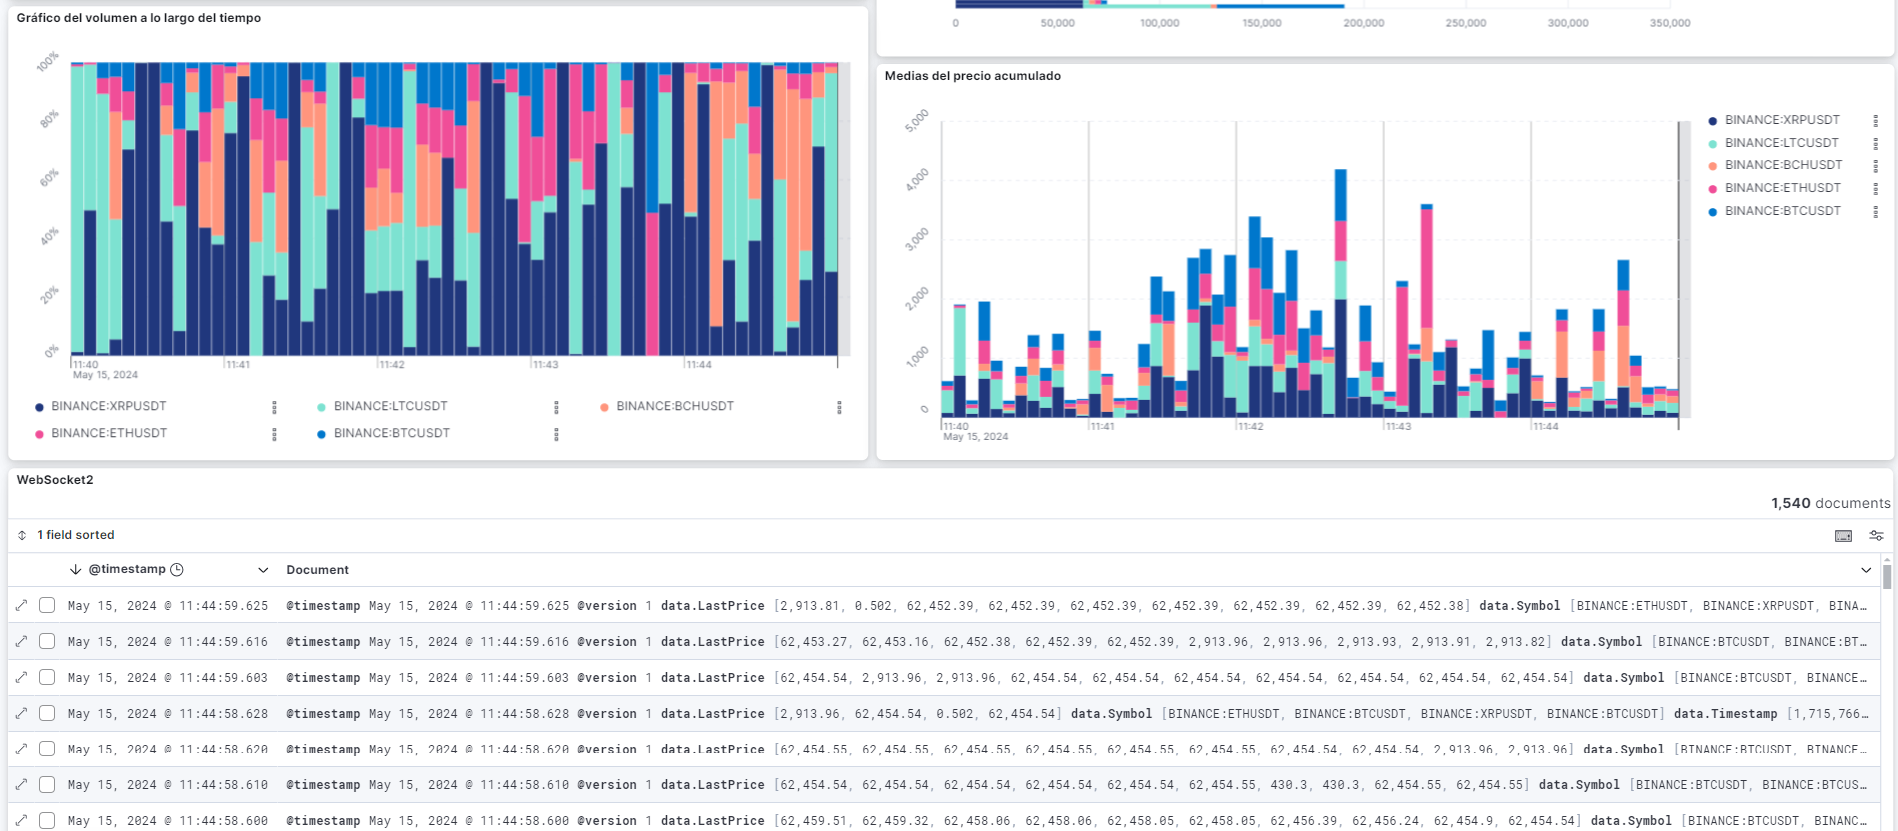
\includegraphics[width=1\linewidth]{img/escenario4-2.png}
    \caption{Dashboard final del cuarto escenario}
    \label{fig:escenario4}
\end{figure}

\paragraph{            }
\paragraph{ }
\paragraph{ }
\paragraph{ }
\paragraph{ }
\paragraph{ }
\paragraph{ }
\paragraph{ }
\paragraph{ }
\paragraph{ }
\paragraph{ }
\paragraph{ }
\paragraph{ }
\paragraph{ }
\paragraph{ }
\paragraph{ }

\subsection{MapReduce para BigData}

En los tiempos que corren, el volumen de transacciones de datos ha aumentado notoriamente, y sigue aumentando a día de hoy. Por lo que los costos de almacenamiento de datos se ha encarecido notablemente. Para reducir estos costes tanto de procesamiento como de almacenamiento, es apropiado utilizar el paradigma de programación  MapReduce, que ya se ha mencionado previamente en los conceptos teóricos. 

Así que una vez se llegó al quinto sprint del proyecto, hubo un enfoque en continuar desarrollando la implementación de MapReduce en una fuente de ingesta de datos sencilla. Por lo que se optó el realizarselo a partir de un fichero de tipo \textit{.log} que contenia distintas transacciones realizadas en una tienda.

\subsubsection{Escenario 5: ingesta de data stream con MapReduce en el servidor mediante Logstash}

En este caso lo que es generar un streaming de datos a partir de un script en Python, cargar esos datos en Logstash, realizarle una serie de modificaciones entre las que se encuentra aplicar el plugin \textit{aggregate}, el cuál cumple el papel de aplicar MapReduce, y cargar esos datos tratados en Elastic para poder visualizarlos en Kibana.

En el data stream sobre el que se va a trabajar, se indican las diferentes transacciones que se han cometido en un comercio con datos sobre las mismas, como el instante de tiempo, el método de pago, la sección en la que se ha comprado, entre otros muchos otros.

Para trabajar con Logstash, se necesita un archivo de configuración para que éste entienda lo que le pedimos que haga. Este archivo es de tipo \textit{.conf} e incluye 3 apartados:
\begin{itemize}
    \item \textbf{Input}: ruta hacia el archivo que contendrá las transacciones
    \item \textbf{Filter}: operaciones a realizarle a estos datos, es decir, el MapReduce con la función \textit{aggregate}
    \item \textbf{Output}: salida por pantalla de los datos mandados a Elastic una vez son tratados.
\end{itemize}

\paragraph{}
\paragraph{}
\paragraph{}


Logstash nos ofrece la función \textit{aggregate}  (ver ilustración  \ref{fig:aggregate}), que permite fusionar muchas líneas de información en una con un determinado criterio en el que se le especifica sobre que campo de los datos va a centrarse. Durante un periodo de tiempo, indicado en la variable \textit{timeout}, la función irá agrupando los registros que concidan con el criterio para que una vez finalizado sean mandados al lugar destino. Se incluirá en el apartado \textit{filter},  indicándole el campo sobre el que hará las agrupaciones en la variable \textit{task id}, así como los datos que se quieren coleccionar una vez son agrupados en la variable \textit{code}. También hay que indicarle un tiempo de inactividad para parar el servicio en la variable \textit{inactivity timeout}.
\begin{figure}
    \centering
    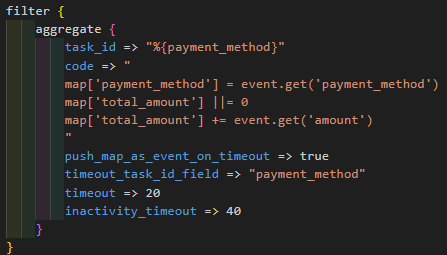
\includegraphics[width=1\linewidth]{img/aggregate.png}
    \caption{Plugin \textit{aggregate} para aplicar MapReduce}
    \label{fig:aggregate}
\end{figure}

En la figura se indica que las agrupaciones se van a realizar en función del método de pago utilizado en cada transacción, y que cada 20 segundos se actualizen estas agrupaciones, y si trás 40 segundos no ha ocurrido ningún cambio, que se detenga el servicio.

En el apartado \textit{output} se indica que los datos procesados seán mandados a ElasticSearch a través del puerto 9200, y que allí se cree un índice con los datos que le lleguen. También se indica que los datos procesados sean mostrados por pantalla para comprobar que todo funciona.

Una vez ejecutado Logstash, a Elastic le llega un índice con tan solo tres filas, las cuáles son las equivalentes a los tres tipos de métodos de pago. Teniendo los datos en el entorno, podemos generar el \textit{dashboard} para mostrarlos y trabajar sobre estas agrupaciones, mostrando el número de compras con cada método de pago en un gráfico de barras horizontal  (ver ilustración  \ref{fig:barras2}), las categorías en las que más se ha gastado  (ver ilustración  \ref{fig:donut2}), los clientes que más han comprado  (ver ilustración  \ref{fig:tabla2}) o el gasto promedio  (ver ilustración  \ref{fig:metrica2}).

\begin{figure}
    \centering
    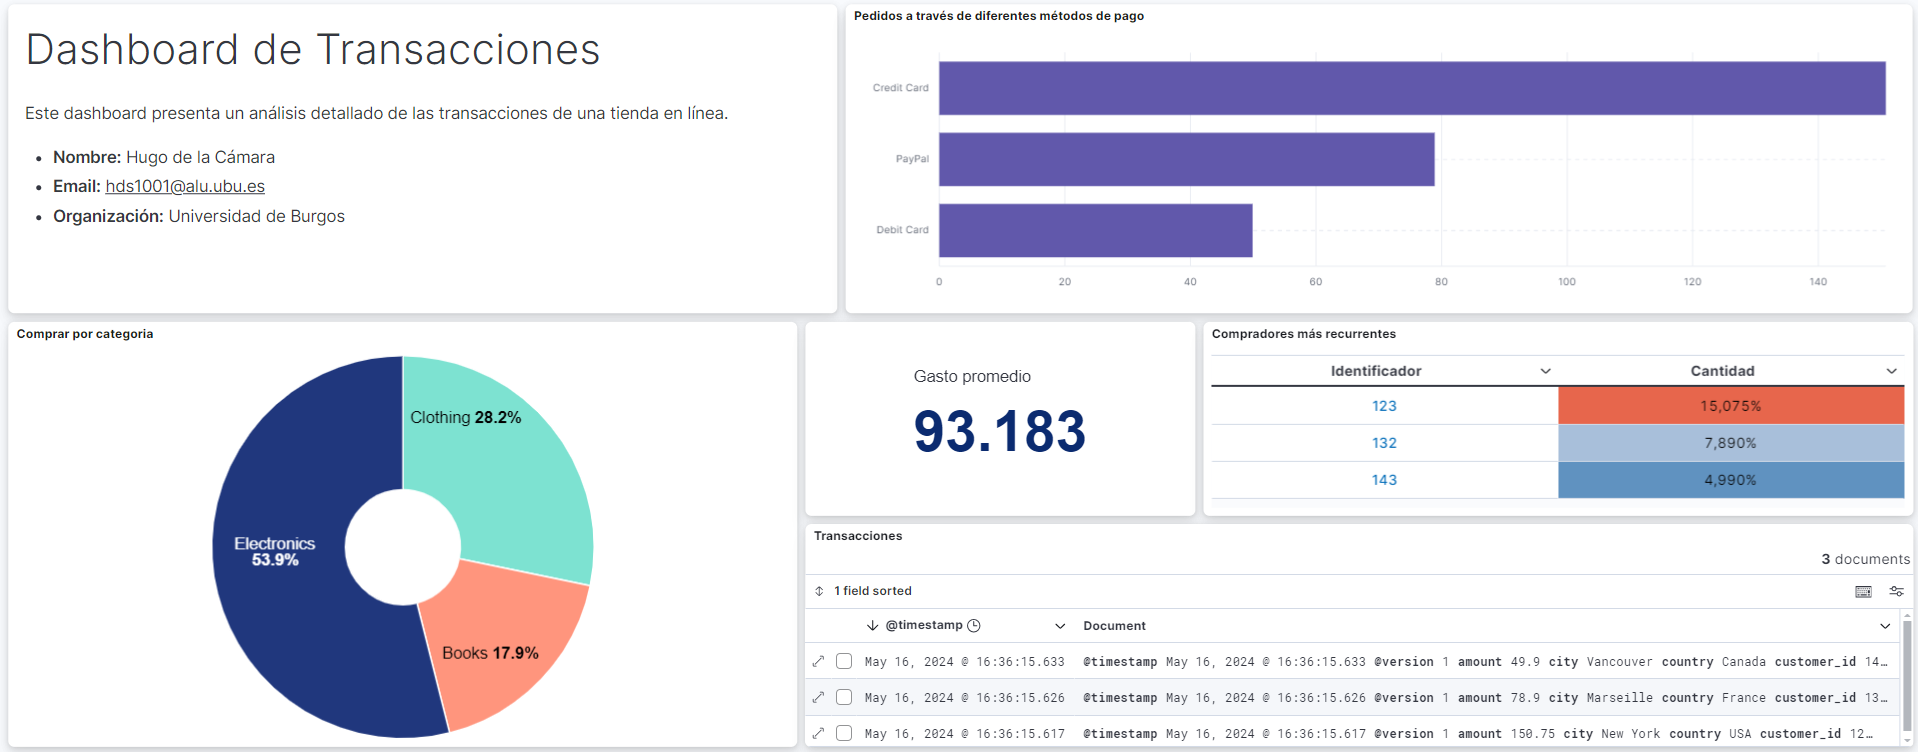
\includegraphics[width=1\linewidth]{img/escenario2.png}
    \caption{Dashboard final del quinto escenario}
    \label{fig:escenario2}
\end{figure}

\begin{figure}
    \centering
    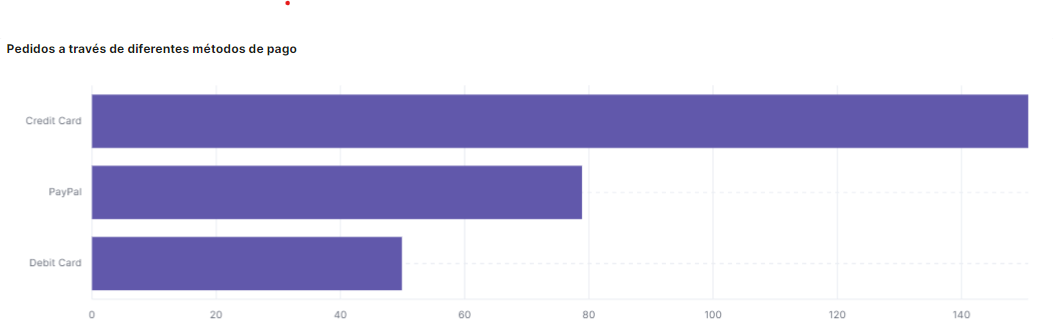
\includegraphics[width=1\linewidth]{img/barras2.png}
    \caption{Gráfico de barras del número de pedidos con cada método de pago}
    \label{fig:barras2}
\end{figure}

\begin{figure}
    \centering
    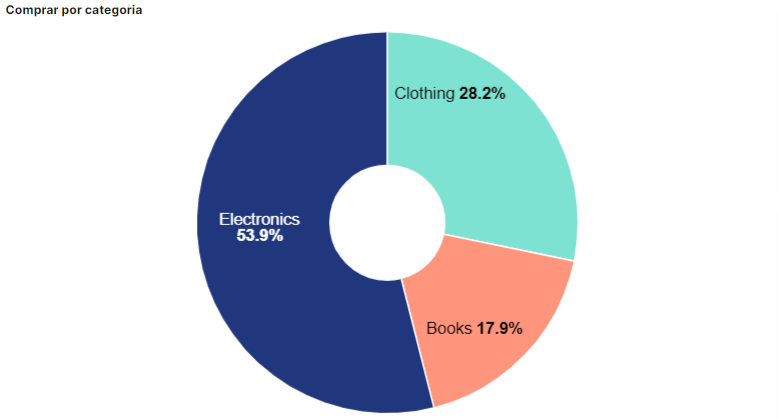
\includegraphics[width=1\linewidth]{img/donut2.png}
    \caption{Gráfico de donut del porcentaje de compra en cada categoría}
    \label{fig:donut2}
\end{figure}

\begin{figure}
    \centering
    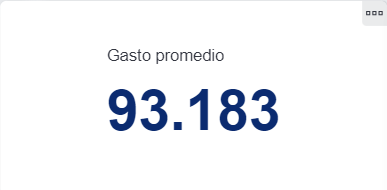
\includegraphics[width=1\linewidth]{img/metrica2.png}
    \caption{Métrica del gasto promedio de cada cliente}
    \label{fig:metrica2}
\end{figure}

\begin{figure}
    \centering
    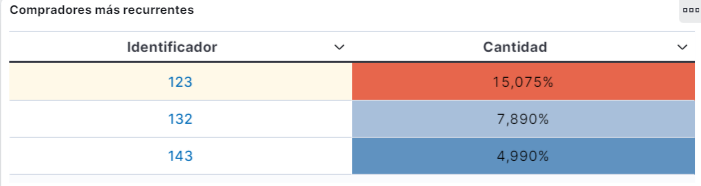
\includegraphics[width=1\linewidth]{img/tabla2.png}
    \caption{Tabla mostrando los clientes más recurrentes}
    \label{fig:tabla2}
\end{figure}


Una vez la carga de los datos en Logstash fue completada con éxito, y se pudo empezar a experimentar con la función que este nos ofrece equivalente a un MapReduce, la función \textit{aggregate}, en la cuál se hizo un agrupado de los datos tomando como referencia el método de pago usado, resultando en que el envío a Elastic fueron 3 lineas con los datos de las cantidades gastadas con cada método y las categorias más compradas entre otros.

\paragraph{}
\paragraph{}

En el caso de este estudio, se aplicó MapReduce a una fuente de datos modesta, puesto que las capacidades de los sistemas en los que se está ejecutando el proyecto son limitadas, pero eso no quita que esta función sea extrapolable a grandes volúmenes de datos con sistemas que sean capaces de procesarlos y reducirlos de cara a moderar el coste de almacenamiento de los mismos. Estos sistemas deben ser clústeres de ordenadores que soporten almacenamiento distribuido , y mediante programas como Hadoop \cite{Hadoop}, esta función se pueda aplicar más fácilmente a grandes masas de datos.

En sistemas de IoT que poseen un gran número de sensores que están mandado datos constantemente es donde resulta interesante aplicar estos conceptos, puesto que se tendrá una estructura ágil para poder analizar la información en tiempo real reduciendo costes.

\paragraph{}
\paragraph{}
\paragraph{}
\paragraph{}
\paragraph{}
\paragraph{}
\paragraph{  }
\paragraph{  }


\subsection{Machine Learning en ELK}

Desde el principio del proyecto se planteó la idea de trabajar con Machine Learning de manera automática con una fuente de ingesta de datos. Al investigar más profundamente, se llegó a la conclusión de que está función si que la ofrece el ecosistema Elastic  (ver ilustración  \ref{fig:machine}), pero pagándola, ya que como se puede observar en la figura las funciones están bloqueadas y solo permite visualizar datos, función que cubre el \textit{Discover}. Hubo que reconducir este escenario de manera que se pudieran aplicar estas técnicas de análisis de manera gratuita.

\begin{figure}
    \centering
    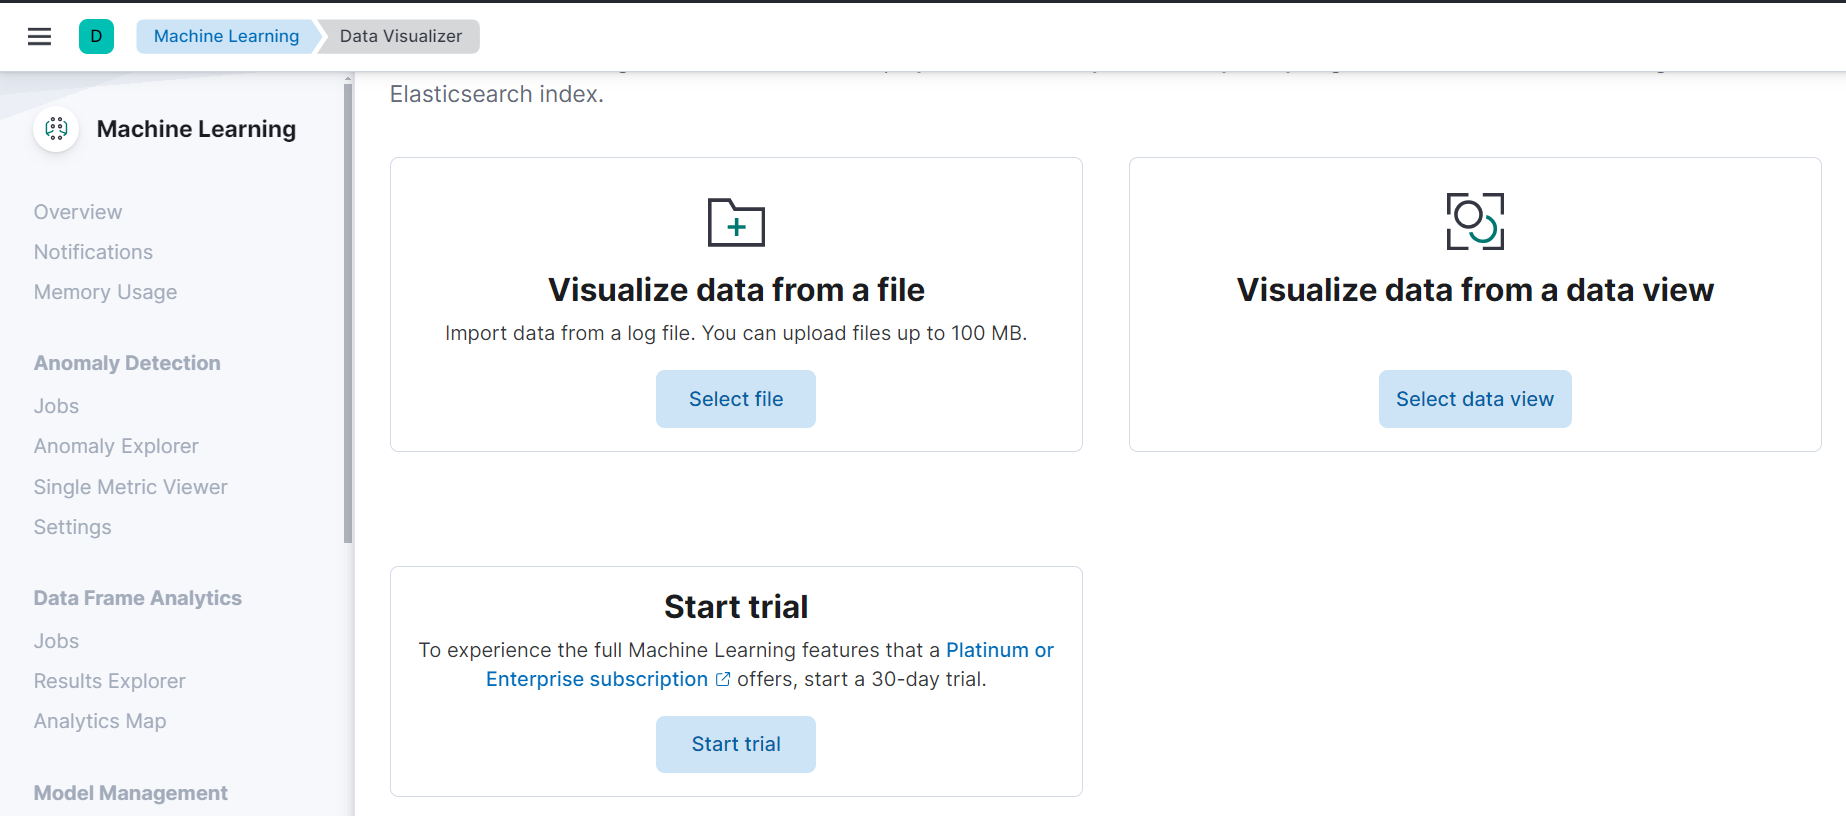
\includegraphics[width=1\linewidth]{img/machineLearning.png}
    \caption{Funcionalidad de Machine Learning de Elastic.}
    \label{fig:machine}
\end{figure}

Y así es como se comenzó a utilizar la biblioteca de análisis predictivo \textit{Scikit-Learn}, la cuál está construida sobre las bibliotecas \textit{Python} de \textit{NumPy}, \textit{SciPy} y \textit{matplotlib}. Para integrar está herramienta en nuestro ecosistema de manera que pudiera interactuar con Elastic, se hizo uso de la herramienta  \textit{Jupyter Notebook}. 

Con \textit{Jupyter}, se generó un script escrito en lenguaje \textit{Python} que importara las librerías necesarias para poder ejecutar los algoritmos de \textit{Scikit-Learn} sobre un conjunto de datos que se le indicara. Como fuente de datos se utilizó un conjunto clásico de las ciencias estadísticas, como lo es el \textit{dataset} Iris, el cuál contiene información sobre tres especies de flores iris, donde cada muestra tiene cuatro características (longitud y anchura del sépalo y del pétalo).

\paragraph{}
\paragraph{}

Lo primero que se hizo fue un script que cargara los datos de Iris en un índice de Elastic, para que un segundo script lea estos desde ese índice, y una vez se tienen los datos cargados en el script desde Elastic, se procede a ejecutar el algoritmo de clasificación \textit{KNN (K vecinos más cercanos)}\cite{knn},  el cuál es un método de clasificación supervisada con el que podemos calcular con qué probabilidad un elemento x desconocido puede pertenecer a una clase a partir de la información que le proporcionemos como prototipo. Una vez se ha obtenido el rendimiento del clasificador, se guardan los resultados localmente en un archivo CSV, y se mandan al puerto 9200 hacia el índice \textit{iris clasificacion}, que será el que almacene los datos en Elastic para que puedan ser mostrados en un \textit{dashboard} de Kibana.

Este proceso de envío de datos va a ser común en los siguientes tres algoritmos que ejecutaremos, siendo el siguiente el de regresión lineal\cite{regresion}, en el cuál se estudia la relación entre la longitud y la anchura de los pétalos de manera que se pueda predecir un comportamiento típico. 

Tras este, vamos a trabajar con algoritmos más visuales, como es el de \textit{clustering} o análisis de grupos con K-Means\cite{clustering} , con el cuál agruparemos los ejemplares de la flor Iris que tengan características similares en diferentes grupos ilustrados con colores. 

Y así concluímos el script con el último algoritmo estudiado, tratándose del de uno reducción de dimensionalidad como es \textit{PCA}\cite{pca}, con el cuál describiremos el conjunto de datos Iris con nuevas variables no correlacionadas, resultando en un gráfico de dispersión bidimensional.

Una vez tenemos toda la información procesada y cargada en Elastic, la creación de un \textit{dashboard} de Kibana viene de la mano, indicándole que los datos se sacarán del índice \textit{Iris} el cuál contiene toda la información que le hemos ido enviando desde el script.

En este \textit{dashboard} se muestran las métricas calculadas por los dos primeros algoritmos  (ver ilustración  \ref{fig:machine1}), y las gráficas calculadas por los dos últimos  (ver ilustraciones  \ref{fig:machine2} y \ref{fig:machine3}, además de información sobre el dataset Iris y los diferentes datos que han cargado los algoritmos como resultado del procesamiento.

\begin{figure}
    \centering
    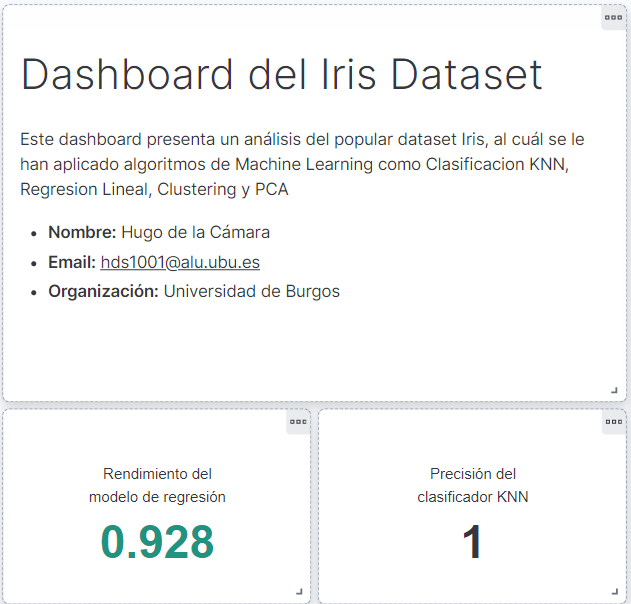
\includegraphics[width=1\linewidth]{img/iris12.png}
    \caption{Visualizaciones mostrando información del \textit{dashboard} así como el rendimiento de la regresión y la precisión del clasificador.}
    \label{fig:machine1}
\end{figure}


\begin{figure}
    \centering
    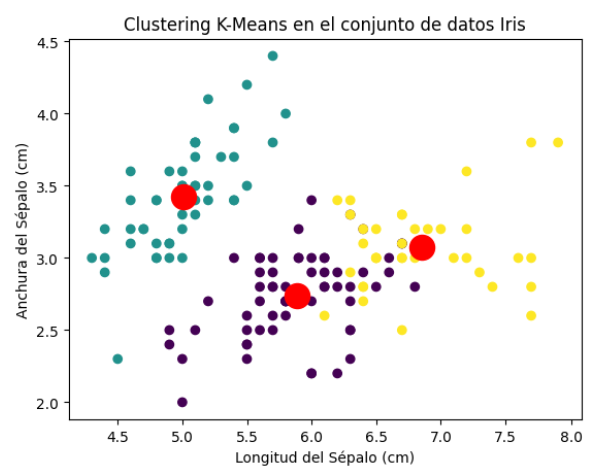
\includegraphics[width=1\linewidth]{img/clustering.png}
    \caption{Visualización de dos dimensiones del gráfico obtenido tras aplicar clustering.}
    \label{fig:machine2}
\end{figure}


\begin{figure}
    \centering
    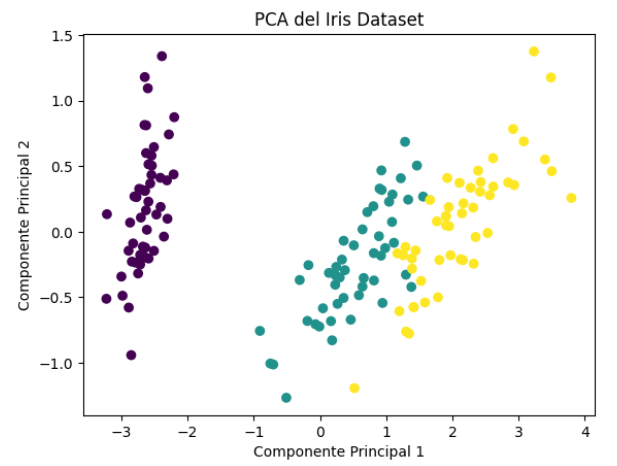
\includegraphics[width=1\linewidth]{img/pca.png}
    \caption{Visualización del gráfico obtenido tras aplicar PCA.}
    \label{fig:machine3}
\end{figure}
